\documentclass[fleqn]{beamer}

\usepackage[czech]{babel}
\usepackage[utf8]{inputenc}
\usepackage[T1]{fontenc}

\usepackage{graphicx}
\usepackage{adjustbox}
\usepackage{caption}

\usetheme{Madrid}

\title{ITY projekt 5 - prezentace IVS}
\author{Josef Michal}
\date{\today}

\begin{document}

\frame{\titlepage}

\begin{frame}{Cíle projektu}
\begin{itemize}
    \item Vytvořit kalkulačku
    \pause
    \begin{itemize}
        \item Uživatelské rozhraní (frontend)
        \item Matematická knihovna
    \pause
    \end{itemize}
    \item Profilovací program pro matematickou knihovnu
    \pause
    \begin{itemize}
        \item Hledání míst pro optimalizaci programu
    \end{itemize}
    \pause
    \item Správná komunikace a spolupráce v týmu
\end{itemize}
\end{frame}









\begin{frame}{Uživatelské rozhraní}
\begin{center}
\begin{minipage}[t]{0.35\linewidth}
    \centering
    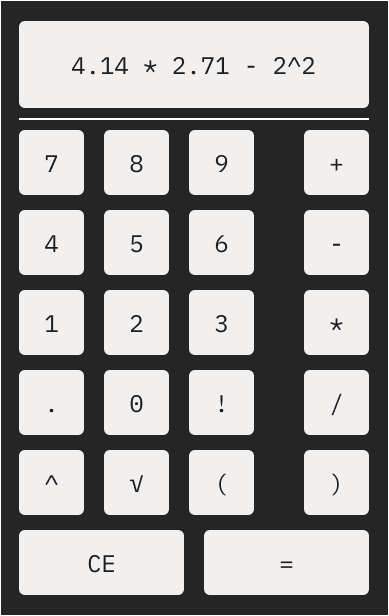
\includegraphics[width=0.9\linewidth]{mockup.png}
    \captionof{figure}{Návrh FE}
\end{minipage}
\pause
\hspace{0.05\textwidth}
\raisebox{3cm}{\Large$\Rightarrow$}
\hspace{0.05\textwidth}
\begin{minipage}[t]{0.35\linewidth}
    \centering
    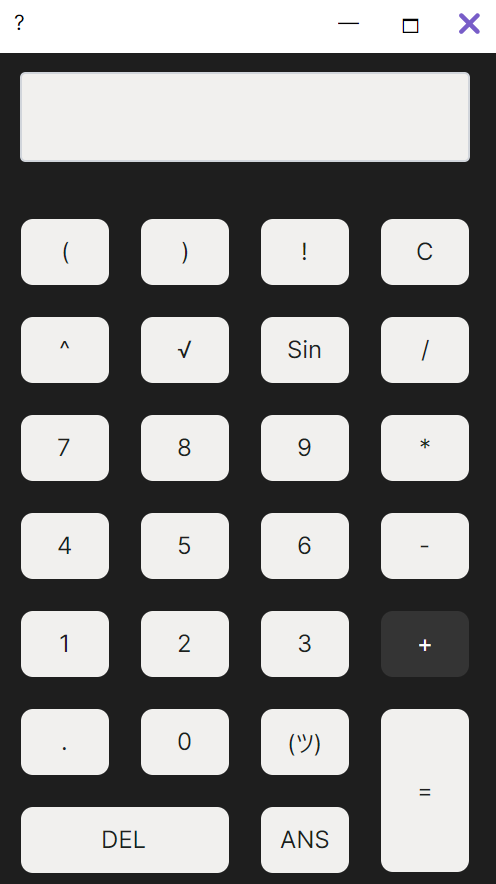
\includegraphics[width=0.9\linewidth]{screenshot.png}
    \captionof{figure}{Finální verze FE}
\end{minipage}
\end{center}

\end{frame}







\begin{frame}{Matematická knihovna}
\begin{itemize}
    \item Rozhraní
    \pause
    \begin{itemize}
        \item Vstup: řetězec
        \item Výstup: desetinné číslo (double)
        \pause
    \end{itemize}
    \item Postup
    \pause
    \begin{itemize}
        \item Parsování vstupu (vytváření tokenů z výrazu)
        \pause
        \item Převod infixové $\Rightarrow$ postfixovou (RPN) notaci
        \pause
        \item Jednodušší vyhodnocení RPN notace
    \end{itemize}
\end{itemize}

\end{frame}










\begin{frame}{Převod infix $\Rightarrow$ postfix}

\begin{itemize}
    \item Zásobník \texttt{S} a výstupní řetězec \texttt{P}\pause
    \item Pro každý symbol $c$ ve vstupním výrazu:\pause
    \begin{itemize}
        \item Pokud je $c$ operand, přidat do \texttt{P}
        \item Pokud je $c$ levá závorka, vložit na zásobník \texttt{S}
        \item Pokud je $c$ pravá závorka:\pause
        \begin{itemize}
            \item Odebírat z \texttt{S} a přidávat do \texttt{P}, do levé závorky\pause
            \item Levou závorku odstranit\pause
        \end{itemize}
        \item Pokud je $c$ operátor:\pause
        \begin{itemize}
            \item Dokud \texttt{S} není prázdný a priorita vrcholu $\geq$ priorita $c$, přesouvat operátory z \texttt{S} do \texttt{P}\pause
            \item Vložit $c$ na zásobník\pause
        \end{itemize}
    \end{itemize}
    \item Po průchodu vstupem: Přesunout všechny zbývající operátory z \texttt{S} do \texttt{P}\pause
    \item Výsledkem je postfixový (RPN) výraz \texttt{P}
\end{itemize}

\end{frame}










\begin{frame}{Profiling}

\begin{itemize}
    \item Výpočet směrodatné odchylky
    \[
    s = \sqrt{\frac{1}{N-1} \left( \sum^{N}_{i=1} x^{2}_{i} - N\overline{x}^2\right)}, \hspace{0.25cm}
    \overline{x} = \frac{1}{N}\sum^{N}_{i=1} x_{i}
    \]
    \pause
    \item Na vstupech velikosti $10^1, 10^3, 10^6$
    \pause
    \item Zacycen pomocí dotnet-trace
\end{itemize}
    
\end{frame}







\begin{frame}{Výstup profilingu}

\begin{itemize}
    \item Pomalé zpracování vstupu
    \begin{itemize}
        \item Hodně času na datových strukturách \pause
        \item \texttt{AddWithResize}, \texttt{PushWithResize}
    \end{itemize}
    \pause
    \item Rychlé zpracování RPN
    \pause
    \item Řešení:
    \pause
    \begin{itemize}
        \item Výběr lepších datových struktur (in-situ?)\pause, nebo
        \item Úplná změna rozhraní knihovny
    \end{itemize}
\end{itemize}
    
\end{frame}






\begin{frame}{Technologie}
\bigskip
\begin{itemize}
    \item Vývoj
    \pause
    \begin{itemize}
        \item C\# + .NET9.0
        \pause
        \item Avalonia Framework
        \begin{itemize}
            \item XAML
        \end{itemize}
        \pause
    \end{itemize}
    \item Verzování
    \pause
    \begin{itemize}
        \item Git\pause
        \item Github
    \end{itemize}
    \pause
    \item Komunikace
    \pause
    \begin{itemize}
        \item Discord
    \end{itemize}
   
\end{itemize}

\end{frame}

\end{document}
